\section{MDD example}
\label{sec:mdd_example}
In this section we provide an example

\begin{figure}[!htb]
	\centering
	\begin{subfigure}[b]{0.95\linewidth}
		\centering
		\centering
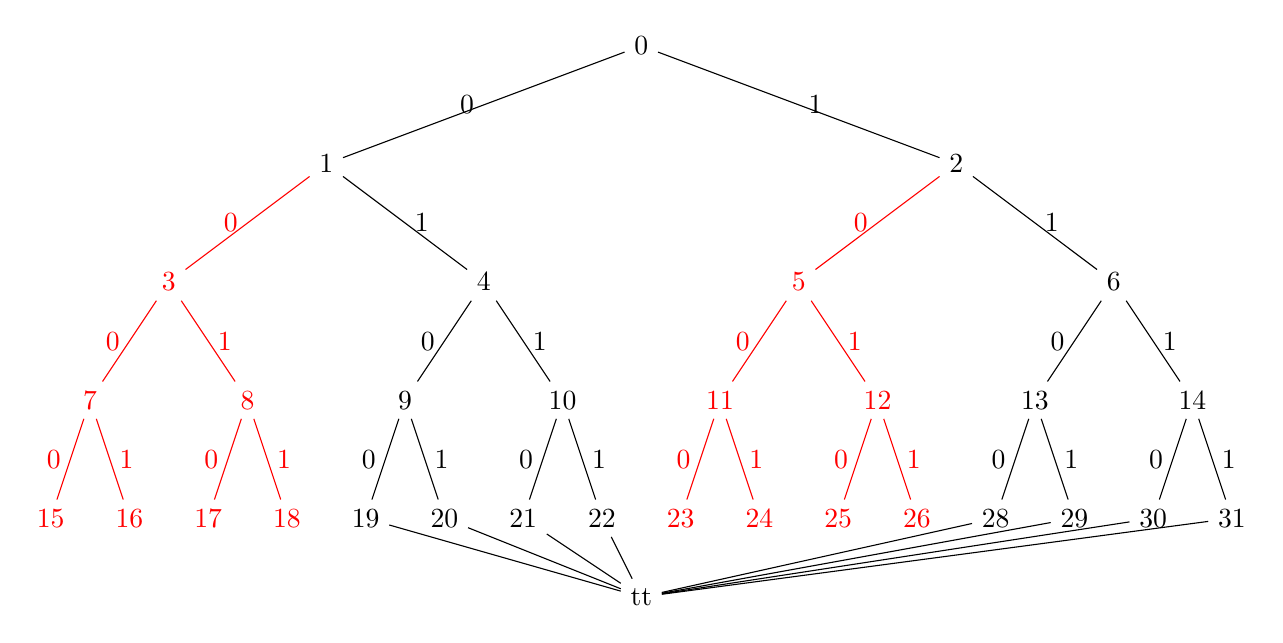
\begin{tikzpicture}
  [
    level 1/.style = {sibling distance = 8cm},
    level 2/.style = {sibling distance = 4cm},
    level 3/.style = {sibling distance = 2cm},
    level 4/.style = {sibling distance = 1cm},
  ]

  \node (root) at (0,0) {0}
  child {node {1}
      child [red] {
          node {3}
          child {node {7}
              child {node {15}
                  edge from parent node [left] {0}}
              child {node {16}
                  edge from parent node [right] {1}}
              edge from parent node [left] {0}}
          child {node {8}
              child {node {17}
                  edge from parent node [left] {0}}
              child {node {18}
                  edge from parent node [right] {1}}
              edge from parent node [right] {1}}
          edge from parent node [left] {0}}
      child {
          node {4}
          child {node {9}
              child {node {19}
                  edge from parent node [left] {0}}
              child {node {20}
                  edge from parent node [right] {1}}
              edge from parent node [left] {0}}
          child {node {10}
              child {node {21}
                  edge from parent node [left] {0}}
              child {node {22}
                  edge from parent node [right] {1}}
              edge from parent node [right] {1}}
          edge from parent node [right] {1}}
      edge from parent node [left] {0}
    }
  child {node {2}
      child [red] {
          node {5}
          child {node {11}
              child {node {23}
                  edge from parent node [left] {0}}
              child {node {24}
                  edge from parent node [right] {1}}
              edge from parent node [left] {0}}
          child {node {12}
              child {node {25}
                  edge from parent node [left] {0}}
              child {node {26}
                  edge from parent node [right] {1}}
              edge from parent node [right] {1}}
          edge from parent node [left] {0}}
      child {node {6}
          child {node {13}
              child {node {28}
                  edge from parent node [left] {0}}
              child {node {29}
                  edge from parent node [right] {1}}
              edge from parent node [left] {0}}
          child {node {14}
              child {node {30}
                  edge from parent node [left] {0}}
              child {node {31}
                  edge from parent node [right] {1}}
              edge from parent node [right] {1}}
          edge from parent node [right] {1}}
      edge from parent node [right] {1}
    };

  \node (bottomnode) at (0,-7) {tt};

  \foreach \w in {1,2}{
      \foreach \x in {1,2} {
          \foreach \y in {1, 2}{
              \draw (root-\w-2-\x-\y) -- (bottomnode);
            }
        }
    }

\end{tikzpicture}
		\caption{Complete \mdd}
		\label{fig:mmd1}
	\end{subfigure}
\end{figure}

\begin{figure}[!htb]\ContinuedFloat
	\begin{subfigure}[b]{.45\linewidth}
		\centering
		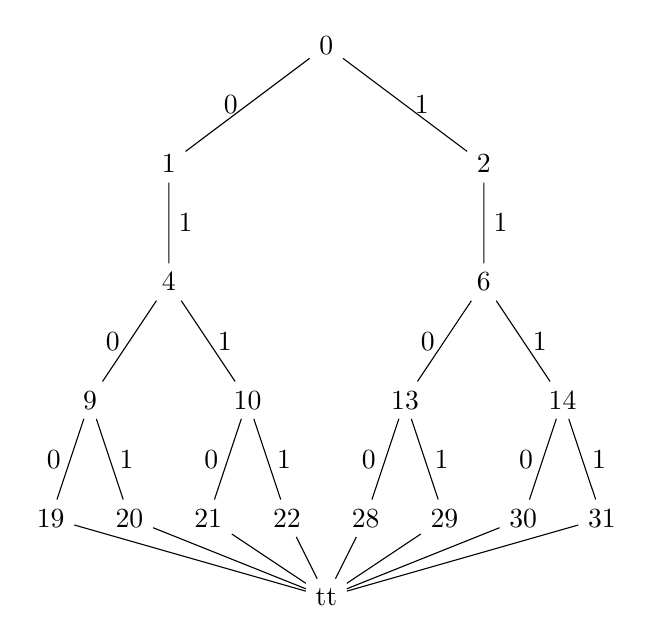
\begin{tikzpicture}
  [
    level 1/.style = {sibling distance = 4cm},
    level 2/.style = {sibling distance = 4cm},
    level 3/.style = {sibling distance = 2cm},
    level 4/.style = {sibling distance = 1cm},
  ]

  \node (root) at (0,0) {0}
  child {node {1}
      child {
          node {4}
          child {node {9}
              child {node {19}
                  edge from parent node [left] {0}}
              child {node {20}
                  edge from parent node [right] {1}}
              edge from parent node [left] {0}}
          child {node {10}
              child {node {21}
                  edge from parent node [left] {0}}
              child {node {22}
                  edge from parent node [right] {1}}
              edge from parent node [right] {1}}
          edge from parent node [right] {1}}
      edge from parent node [left] {0}
    }
  child {node {2}
      child {node {6}
          child {node {13}
              child {node {28}
                  edge from parent node [left] {0}}
              child {node {29}
                  edge from parent node [right] {1}}
              edge from parent node [left] {0}}
          child {node {14}
              child {node {30}
                  edge from parent node [left] {0}}
              child {node {31}
                  edge from parent node [right] {1}}
              edge from parent node [right] {1}}
          edge from parent node [right] {1}}
      edge from parent node [right] {1}
    };

  \node (bottomnode) at (0,-7) {tt};

  \foreach \w in {1,2}{
      \foreach \x in {1,2} {
          \foreach \y in {1, 2}{
              \draw (root-\w-1-\x-\y) -- (bottomnode);
            }
        }
    }

\end{tikzpicture}
		\caption{Reduction $1$}
		\label{fig:mmd2}
	\end{subfigure}
	\hfill
	\begin{subfigure}[b]{.45\linewidth}
		\centering
		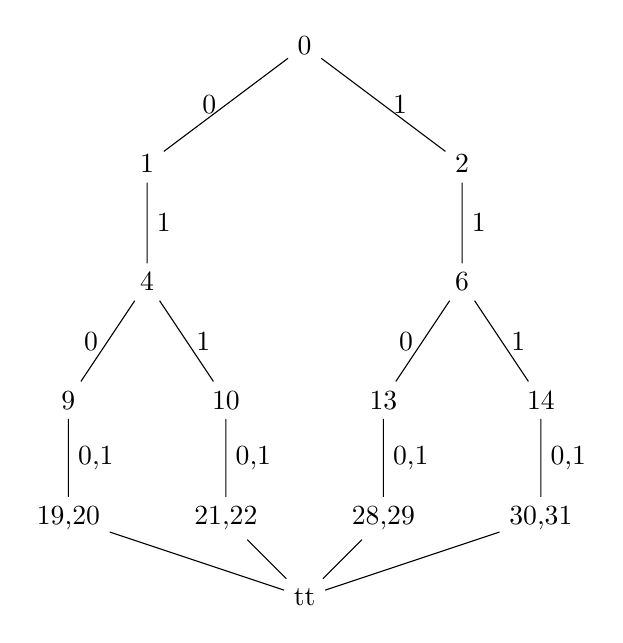
\begin{tikzpicture}
  [
    level 1/.style = {sibling distance = 4cm},
    level 2/.style = {sibling distance = 2cm},
    level 4/.style = {sibling distance = 1cm},
  ]

  \node (root) at (0,0) {0}
  child {node {1}
      child {
          node {4}
          child {node {9}
              child {node {19,20}
                  edge from parent node [right] {0,1}}
              edge from parent node [left] {0}}
          child {node {10}
              child {node {21,22}
                  edge from parent node [right] {0,1}}
              edge from parent node [right] {1}}
          edge from parent node [right] {1}}
      edge from parent node [left] {0}
    }
  child {node {2}
      child {node {6}
          child {node {13}
              child {node {28,29}
                  edge from parent node [right] {0,1}}
              edge from parent node [left] {0}}
          child {node {14}
              child {node {30,31}
                  edge from parent node [right] {0,1}}
              edge from parent node [right] {1}}
          edge from parent node [right] {1}}
      edge from parent node [right] {1}
    };

  \node (bottomnode) at (0,-7) {tt};

  \foreach \w in {1,2}{
      \foreach \x in {1,2} {
          \draw (root-\w-1-\x-1) -- (bottomnode);
        }
    }

\end{tikzpicture}
		\caption{Reduction $2$}
		\label{fig:mmd3}
	\end{subfigure}
\end{figure}

\begin{figure}[!htb]\ContinuedFloat
	\begin{subfigure}[b]{.45\linewidth}
		\centering
		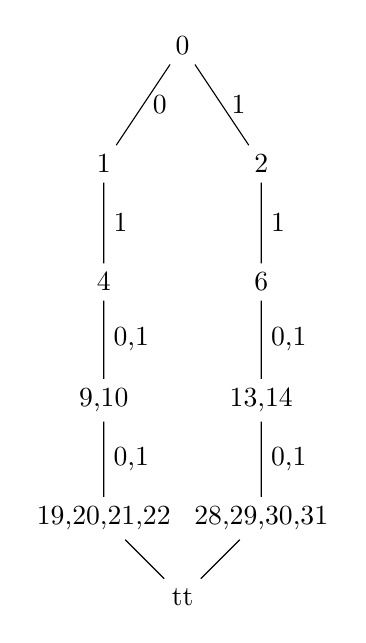
\begin{tikzpicture}
    [
        level 1/.style = {sibling distance = 2cm},
    ]

    \node (root) at (0,0) {0}
    child {node {1}
            child {
                    node {4}
                    child {node {9,10}
                            child {node {19,20,21,22}
                                    edge from parent node [right] {0,1}}
                            edge from parent node [right] {0,1}}
                    edge from parent node [right] {1}}
            edge from parent node [right] {0}
        }
    child {node {2}
            child {node {6}
                    child {node {13,14}
                            child {node {28,29,30,31}
                                    edge from parent node [right] {0,1}}
                            edge from parent node [right] {0,1}}
                    edge from parent node [right] {1}}
            edge from parent node [right] {1}
        };

    \node (bottomnode) at (0,-7) {tt};

    \foreach \w in {1,2}{
            \draw (root-\w-1-1-1) -- (bottomnode);
        }

\end{tikzpicture}
		\caption{Reduction $3$}
		\label{fig:mmd4}
	\end{subfigure}
	\hfill
	\begin{subfigure}[b]{.45\linewidth}
		\centering
		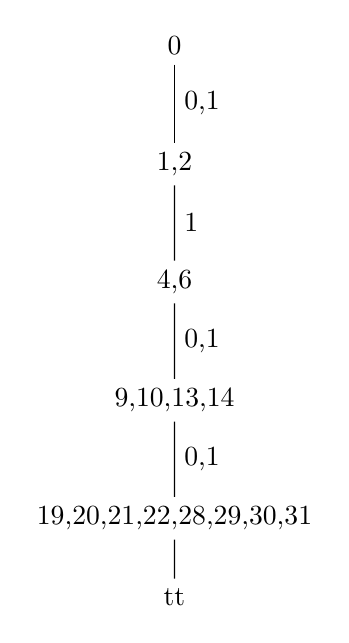
\begin{tikzpicture}

  \node (root) at (0,0) {0}
  child {node {1,2}
      child {
          node {4,6}
          child {node {9,10,13,14}
              child {node {19,20,21,22,28,29,30,31}
                  edge from parent node [right] {0,1}}
              edge from parent node [right] {0,1}}
          edge from parent node [right] {1}}
      edge from parent node [right] {0,1}
    };

  \node (bottomnode) at (0,-7) {tt};

  \draw (root-1-1-1-1) -- (bottomnode);

\end{tikzpicture}
		\caption{Final reduction}
		\label{fig:mmd5}
	\end{subfigure}

	\caption{\mdd\ for $\mathcal{L} = \{\omega \in \{0, 1\}^4 \mid \omega[2] = 1\}$}
	\label{fig:mmd}
\end{figure}